% !TEX root = ./notes.tex
\chapter{Nuclear Physics}

\section{The Nuclear Landscape}

From nucleon-nucleon scattering, we find that the nuclear force operates over a range of $\lesssim 2\ee{-13}\nsp\cm \equiv 2\nsp\fermi$, where $\fermi$ denotes the unit of length known as a ``fermi.''  At low energies the nuclear force can be described as the exchange of spin-zero pions; recall from quantum field theory that  the exchange of a spin-zero particle produces an attractive potential of the form $\sim (1/r)e^{-r/\lambda_{\pi}}$, where $\lambda_{\pi} = \hbar/(m_{\pi}c)$ is the Compton wavelength of the force carrier. The pion rest mass is $\approx 140\nsp\MeV/c^{2}$, so $\lambda_{\pi} \approx 1.4\nsp\fermi$.  The nuclear force is indeed attractive over this range,  but it becomes repulsive at distances $< 1\nsp\fermi$ where the simple pion exchange model breaks down.  This attractive interaction with a repulsive core resembles the interaction between molecules in a fluid.  Indeed, for heavy nuclei, the nucleons form a ``nuclear fluid'' with a characteristic density of $0.16\nsp\fermi^{-3}$.  The \textbf{binding energy} is defined as
\begin{equation}\label{e.binding-energy-def}
B(N,Z) = \left[Z m_{p} + N m_{n} - M(N,Z)\right] c^{2},
\end{equation}
where $M$ is the total mass of a nucleus with $N$ neutrons and $Z$ protons. The total number of nucleons is $A = N+Z$, the proton rest mass is $m_{p} = 938.272\nsp\MeV/c^{2}$, and the neutron rest mass is $m_{n} = 939.565\nsp\MeV/c^{2}$.
From the form of this definition $B > 0$ for bound nuclei and is $\approx 8\nsp\MeV$. The fact that the nuclear interaction binds the nucleons into a ``nuclear fluid'' means that one can make a crude model of the nucleus as a liquid drop, and use this model to fit the binding energy.
This model, due to Weiz\"acker, is
\begin{equation}\label{e.weizacker-fmla}
-B(N, Z) = a_{V} A + a_{S}A^{2/3} + a_{A}\frac{(N-Z)^{2}}{A} + a_{C}\frac{Z^{2}}{A^{1/3}} + a_{p}\delta A^{-1/2},
\end{equation}
and has four terms: a bulk energy term $a_{V}A$ that scales with the total number of nucleons; a surface term $a_{S}A^{2/3}$ that corrects for the weaker binding near the surface; an asymmetry term $a_{A}(N-Z)^{2}/A$ that accounts for the energy cost to have an imbalance in the number of neutrons and protons; and a Coulomb term $a_{C}Z^{2}/A^{1/3}$ that accounts for the repulsion between other protons.  
 The quantity $\delta$ describes the pairing:
\[
\delta = \left\{\begin{array}{lr}+1,& \textrm{$N$, $Z$ even;} \\-1,& \textrm{$N$, $Z$ odd;} \\ 0,& \textrm{$N$ even, $Z$ odd, or $N$ odd, $Z$ even}\end{array}\right. .
\]
Using the online fitting routine from the \href{http://128.95.95.61/~intuser/ld.html}{Institute for Nuclear Theory}, I obtained the coefficients listed in Table~\ref{t.liquid-drop}.

\begin{table}[htbp]
\label{t.liquid-drop}
\caption{Coefficients for the Weiz\"acker mass formula.\label{t.liquid-drop-coefficients}}
\begin{center}
\begin{tabular}{l|rrrrr}
\hline
coefficient & $a_{V}$ & $a_{S}$ & $a_{A}$ & $a_{C}$ & $a_{p}$ \\
\hline\hline
value (MeV) & -15.67 & 17.04 & 23.09 & 0.71 & -14.55\\
\hline
\end{tabular}
\end{center}
\end{table}

This simple formula gives a good, if somewhat crude, description of the nuclear landscape.  As a first example,  let's look at how the binding energy per nucleon, $-B/A$ trends with $A$.  For simplicity, we'll ignore the pairing term. Dividing equation~(\ref{e.weizacker-fmla}) by $A$, and denoting the neutron asymmetry by $\eta \equiv (N-Z)/(N+Z)$, we obtain
\begin{equation}\label{e.binding-energy-per-nucleon}
 -\frac{B}{A} = a_{V} + a_{S} A^{-1/3} + a_{A}\eta^{2} + \frac{a_{C}}{4} \left( 1-\eta\right)^{2} A^{2/3}.
\end{equation}
Minimizing this expression for small $A$, we see that the most bound nuclei (smallest $-B/A$) have $\eta \to 0$, i.e., equal numbers of neutrons and protons.  As $A$ increases, however, the Coulomb term becomes important.  Expanding the last two terms and combining gives the sum of the asymmetry and Coulomb terms,
\[ \frac{a_{C}}{4} A^{2/3} - \frac{a_{C}}{2}A^{2/3}\eta + \left[ \frac{a_{C}}{4}A^{2/3} + a_{A} \right] \eta^{2} .\]
For large $A$, this expression is minimized (although it cannot be made to vanish) for $\eta > 0$: that is, $N>Z$ and the most bound massive nuclei are neutron-rich. The nuclei for which $-B/A$ is a minimum for a fixed $A$ define the \emph{valley of stability}. How does the binding energy change with $A$ along this valley?  At small $A$, the asymmetry term dominates and $\eta^{2}\ll 1$.  As $A$ increases, the surface term $a_{S}A^{-1/3}$ becomes smaller and $B/A$ increases.  At large $A$, however, the sum of the Coulomb and asymmetry terms decreases $B/A$.  As a result, there is a peak in $B/A$, which is around $A = 56$.

Next, let's find the boundaries of our nuclear landscape: the most neutron-rich and proton-rich nuclei that are still bound.
Define the \textbf{neutron separation energy} $S_{n}$ as the energy needed to remove a neutron from a nucleus,
\begin{eqnarray}\label{e.Sn}
S_{n}(N,Z) &\equiv& c^{2}\left\{\left[M(N-1,Z) + m_{n}\right] - M(N,Z)\right\} \nonumber\\
	&=& B(N,Z) - B(N-1,Z).
\end{eqnarray}
Likewise, define the \textbf{proton separation energy} as
\begin{eqnarray}\label{e.Sp}
S_{p}(N,Z) &\equiv& c^{2}\left\{\left[M(N,Z-1) + m_{p}\right] - M(N,Z)\right\} \nonumber\\
	&=& B(N,Z) - B(N,Z-1).
\end{eqnarray}
If we take a nucleus $(N,Z)$ in the valley of stability and add protons keeping $N$ fixed, we will eventually reach a nucleus for which $S_{p} = 0$, that is, it costs no energy to add or to remove a proton.  This defines the \textbf{proton-drip line}: nuclei more proton-rich are unstable to proton emission. Likewise, on the neutron-rich side there is the \textbf{neutron-drip line}, for which $S_{n} = 0$.

\section{Non-resonant nuclear reactions}

The situation we are interested in is the reaction between two nuclei, $(A_{1},Z_{1})$ and $(A_{2},Z_{2})$.  The nuclear radius is $\rn\approx  A^{1/3}\nsp\fermi$, and the Coulomb energy at this distance is
\begin{equation}\label{e.cb}
\frac{Z_{1}Z_{2}e^{2}}{\rn} = \frac{Z_{1}Z_{2}\alpha \hbar c}{ \rn} \approx 1.4 Z_{1}Z_{2}A^{-1/3}\nsp\MeV\gg kT.
\end{equation}
For nuclear reactions, typical energy scales  are $\sim\MeV$ and typical length scales are $\sim\fermi$.  In these units, $\hbar c = 197 \nsp\MeV\usp\fermi$.  In the first equality in eq.~(\ref{e.cb}), we introduce the fine-structure constant $\alpha = e^{2}/(\hbar c) = 1/137$; In ``nuclear units,'' $e^{2} = \alpha \hbar c = (197\nsp\MeV\usp\fermi)/137 = 1.44\nsp\MeV\usp\fermi$. Remember these numbers!  If we scatter two nuclei together, the closest approach (cf.~\S\ref{s.plasma-collisions}) is $\sim e^{2}/(\kB T) \sim 1440\nsp\fermi$ at typical stellar energies $\kB T \sim 1\nsp\keV$.
Clearly the cross-section for a reaction between our pair of particles is controlled by the probability of tunneling through the Coulomb potential.

For a two-body system, it is convenient to transform into a center-of-mass frame.  Our problem then reduces to a one-body problem with reduced mass $m = A\mb$, with $A=A_{1}A_{2}/(A_{1}+A_{2})$ and incident energy $E = m v^{2}/2$, where $v$ is the relative velocity of the two particles.  For now, we'll neglect angular momentum ($\ell = 0$) so our scattering is s-wave.
At low energies, we can form a ``geometrical'' cross-section from the particle wavenumber $k = p/\hbar$, with
\begin{equation}\label{e.geo}
\pi k^{-2} = \pi\frac{\hbar^{2}}{(2mE)} = 660\nsp\barn\frac{1}{A}\left(\frac{\keV}{E}\right)
\end{equation}
Here the cross-section is in units of \emph{barns}, with $1\nsp\barn = 10^{-24}\nsp\cm^{2}$.  This is the first part of our nuclear cross-section $\sigma(E)$. 

The second portion of the nuclear cross-section is the probability of tunneling through the Coulomb barrier.  First, let's get the classical turning point \re\ from
\begin{eqnarray}
\frac{Z_{1}Z_{2}e^{2}}{\re} &=& E,\nonumber\\
\re &=& 1440\nsp\fermi\nsp Z_{1}Z_{2}\left(\frac{\keV}{E}\right).
\end{eqnarray}
Now the wavelength is $k^{-1} = \hbar(2A\mb E)^{-1/2} = \hbar c (2A\mb c^{2} E)^{-1/2}$ and since $\mb c^{2} = 932\nsp\MeV$ the wavelength $k^{-1} = 145\nsp\fermi\usp(\keV/E)^{1/2}$. The important point is that since $k^{-1}\ll \re$, we can solve the Schr\"odinger equation using the WKB approximation.

The WKB approximation is standard, so let me just remind you that the probability of tunneling through the barrier depends on the \emph{action},
\begin{equation}\label{e.wkb}
\mathcal{P} \propto \exp\left\{\frac{2}{\hbar}\int_{\re}^{\rn}\left[2m\left(\frac{Z_{1}Z_{2}e^{2}}{r}-E\right) \right]^{1/2}\,\dif r\right\}.
\end{equation}
To do this integral, note that $\re\gg\rn$, so we can make the approximation $\rn\to 0$ and change variables to
\[
\sin\phi = \left[2m\left(\frac{Z_{1}Z_{2}e^{2}}{r}-E\right) \right]^{1/2}\frac{r}{2mZ_{1}Z_{2}e^{2}};
\]
with this substitution we tame the integral and obtain
\begin{equation}\label{e.prob}
\mathcal{P} \propto \exp\left\{-\frac{8mZ_{1}Z_{2}e^{2}}{\hbar(2mE)^{1/2}}\int_{0}^{\pi/2}\sin^{2}\phi\,\dif\phi\right\} = \exp\left[-\left(\frac{\EG}{E}\right)^{1/2}\right],
\end{equation}
where
\begin{equation}\label{e.EGamow}
\EG\equiv 2\pi^{2} A \mb c^{2} \alpha^{2} (Z_{1}Z_{2})^{2} = 979\nsp\keV \nsp A (Z_{1}Z_{2})^{2}
\end{equation}
is the \emph{Gamow energy}.  Note the strong dependence on $Z_{1}Z_{2}$: \EG\ determines which reactions can occur at a given temperature. If you stare at the factor multiplying the integral in equation~(\ref{e.prob}), you will see that $\mathcal{P}\propto \exp(-\re/\lambda)$, the exponential of ratio of the width of the forbidden region to the wavelength of the incident particle. This makes intuitive sense.

Now we have the second part of our cross-section, the probability of getting through the Coulomb barrier.  This third part depends on the nuclear interactions.  For non-resonant reactions, this third part does not depend strongly on energy, so it is common to define the \emph{astrophysical S-factor} by writing the cross section as the product $(\textrm{geometrical})\times(\textrm{tunneling})\times(\textrm{nuclear})$, 
\begin{equation}\label{e.s-def}
\sigma(E) = \frac{1}{E}\exp\left[-\left(\frac{\EG}{E}\right)^{1/2}\right] S(E).
\end{equation}
It is easier to extrapolate the slowly varying $S(E)$ from lab energies of $> 100\nsp\keV$ down to center-of-mass energies of $\sim \keV$ than it would be to fit the rapidly varying cross-section.

Now each nucleus has a Maxwellian velocity distribution,
\begin{equation}\label{e.maxwell}
n_{1}(\bvec{v}_{1})\,\dif^{3}v = n_{1}\left(\frac{m_{1}}{2\pi kT}\right)^{3/2}\exp\left(-\frac{mv^{2}}{2kT}\right) \,\dif^{3}v,
\end{equation}
and similarly for particle 2.  Let's call a particular nucleus 1 (having velocity $\bvec{v}_{1}$) the target. By definition the cross section is 
\[ \frac{\textrm{number of reactions}/\textrm{target}/\textrm{time}}{\textrm{number of incident particles}/\textrm{area}/\textrm{time}},
\]
so to get the number of reactions per target per time we need to multiply $\sigma(E)$ by the number of incident particles per unit area per unit time.  The incident flux is just $n_{2}(\bvec{v}_{2})|\bvec{v}|\,\dif^{3}v_{2}$ where $\bvec{v}=\bvec{v}_{2}-\bvec{v}_{1}$.  Hence the reaction rate per unit volume per unit time between a pair of particles having velocities in volumes $\dif^{3}v_{1}$ and $\dif^{3}v_{2}$ about $\bvec{v}_{1}$ and $\bvec{v}_{2}$ is just
\[
\frac{1}{1+\delta_{12}} n_{1}(\bvec{v}_{1})n_{2}(\bvec{v}_{2})\sigma(E)|\bvec{v}| \,\dif^{3}v_{1}\dif^{3}v_{2}.
\]
The factor $(1+\delta_{12})^{-1}$ is equal to $1/2$ if particles 1 and 2 are identical, and is there to avoid double-counting in that case. To get the total reaction rate per unit time, we need to integrate over the joint velocity distribution $\dif^{3}v_{1}\,\dif^{3}v_{2}$,
\begin{eqnarray}\label{e.rate-joint}
\lefteqn{r_{12} = \frac{n_{1}n_{2}}{1+\delta_{12}}  \left[\frac{m_{1}m_{2}}{(2\pi kT)^{2}}\right]^{3/2}}
  \nonumber\\ &&\times\int\! \sigma(E) v\exp\left(-\frac{m_{1}v_{1}^{2}}{2kT}-\frac{m_{2}v_{2}^{2}}{2kT}\right)  \,\dif^{3} v_{1}\,\dif^{3}v_{2}.
\end{eqnarray}
Now $E$ and $v$ are the relative energies and velocity in the center-of-mass frame.  We can change variable using the relations
\begin{eqnarray*}
\bvec{v}_{1} &=& \bvec{V} - \frac{m_{2}}{m_{1}+m_{2}} \bvec{v}\\
\bvec{v}_{2} &=& \bvec{V} + \frac{m_{1}}{m_{1}+m_{2}} \bvec{v}.
\end{eqnarray*}
where $V$ is the center-of-mass velocity. It is straightforward to show that $\dif v_{1,x}\,\dif v_{2,x} = \dif V_{x}\dif v_{x}$, and likewise for the $y,z$ directions.  Furthermore, $m_{1}v_{1}^{2} + m_{2}v_{2}^{2} = (m_{1}+m_{2})V^{2} + m v^{2}$, and multiplying and dividing the integral in equation~(\ref{e.rate-joint}) by $m_{1}+m_{2}$ allows us to write
\begin{eqnarray*}
\lefteqn{r_{12} = \frac{n_{1}n_{2}}{1+\delta_{12}} \left(\frac{m_{1}+m_{2}}{2kT}\right)^{3/2}\left(\frac{m}{2kT}\right)^{3/2}}\\
&&\times \int\!\dif^{3}V \int\!\dif^{3}v \,\sigma(E)v \exp\left[-\frac{mv^{2}}{2kT}\right]
 \exp\left[-\frac{(m_{1}+m_{2})V^{2}}{2kT}\right].
\end{eqnarray*}
The integral over $\dif^{3}V$ can be factored out and is normalized to unity. Hence we have for the reaction rate between a pair of particles 1 and 2, 
\begin{eqnarray}\label{e.rate}
r_{12} &=& \frac{1}{1+\delta_{12}}n_{1}n_{2}\left\{\left(\frac{m}{2\pi kT}\right)^{3/2}\int_{0}^{\infty}\! \sigma(E) v \exp\left(-\frac{mv^{2}}{2kT}\right)  4\pi v^{2}\,\dif v\right\}.\nonumber\\
 &\equiv& \frac{1}{1+\delta_{12}}n_{1}n_{2}\langle\sigma v\rangle.
\end{eqnarray}
The term in $\{\}$ is the averaging over the joint distribution of the cross-section times the velocity, and is usually denoted as $\langle\sigma v\rangle$. 

Changing variables to $E = mv^{2}/2$ in equation~(\ref{e.rate}) and inserting the formula for the cross-section, equation~(\ref{e.s-def}), gives
\begin{equation}\label{e.integral}
\langle\sigma v\rangle = \left(\frac{8}{\pi m}\right)^{1/2}\left(\frac{1}{kT}\right)^{3/2}\int_{0}^{\infty}\!S(E)\exp\left[-\left(\frac{\EG}{E}\right)^{1/2}-\frac{E}{kT}\right]\,\dif E.
\end{equation}
Now, we've assumed that $S(E)$ varies slowly; but look at the argument of the exponential. This is a competition between a rapidly rising term $\exp[-(\EG/E)^{1/2}]$ and a rapidly falling term $\exp(-E/kT)$. As a result, the exponential will have a strong peak, and we can expand the integrand in a Taylor series about the maximum. Let 
\[
f(E) = -\left(\frac{\EG}{E}\right)^{1/2} - \frac{E}{kT}.
\]
Then we can write 
\begin{eqnarray*}
\lefteqn{\int_{0}^{\infty}\!S(E)\exp\left[-\left(\frac{\EG}{E}\right)^{1/2}-\frac{E}{kT}\right]\,\dif E}\\
&\approx&
	\int_{0}^{\infty}\! S(\Epk)\exp\left[f(\Epk) + \frac{1}{2}\left.\frac{\dif^{2} f}{\dif E^{2}}\right|_{E=\Epk}\left(E-\Epk\right)^{2}\right].
\end{eqnarray*}
Here $\Epk$ is found by solving $(\dif f/\dif E)|_{E=\Epk} = 0$. This trick allows us to turn the integral into a Gaussian! (Before the internet, all there was to do for fun were integrals.)

Solving for \Epk, we get
\[
\Epk = \frac{\EG^{1/3}(kT)^{2/3}}{2^{2/3}},
\]
and 
\[ \exp\left[f(\Epk)\right] = \exp\left[-3\left(\frac{\EG}{4kT}\right)^{1/3}\right].
\]
Further,
\[
\left.\frac{1}{2}\frac{\dif^{2}f}{\dif E^{2}}\right|_{E=\Epk} = -\frac{3}{2(2\EG)^{1/3}(kT)^{5/3}} = -\frac{3}{4\Epk kT}.
\]
Defining a variable $\Delta = 4(\Epk kT/3)^{1/2}$, our integral becomes
\begin{eqnarray}\label{e.integral2}
\lefteqn{\langle\sigma v\rangle = \left(\frac{8}{\pi m}\right)^{1/2}\left(\frac{1}{kT}\right)^{3/2}}\nonumber\\
&&\times S(\Epk)
  \exp\left[-3\left(\frac{\EG}{4kT}\right)^{1/3}\right]
  \int_{0}^{\infty}\!\exp\left[-\frac{(E-\Epk)^{2}}{(\Delta/2)^{2}}\right]\,\dif E.
\end{eqnarray}
How well does this approximation do?  Figure~\ref{f.integrand} shows the integrand (\emph{solid line}) and the approximation by a Gaussian (\emph{dashed line}).  Although the integrand is skewed to the right, the area is approximately the same.  We could correct for this by taking more terms in our expansion. Consult Clayton for details.

\begin{figure}[htbp]
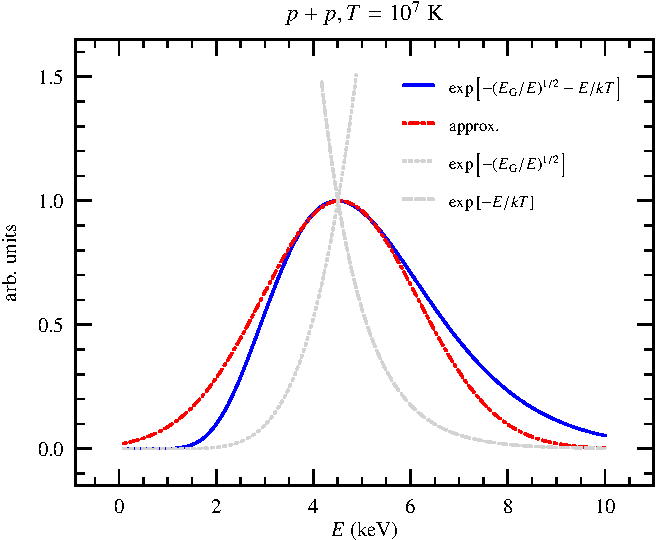
\includegraphics[width=4in]{Figures/plots_out/coulomb_integrand}
\caption{Integrand of eq.~(\protect\ref{e.integral}) (\emph{solid line}) and the Gaussian (\emph{dot-dashed line}) constructed by expanding to second order the argument of the exponential. The parameters for $\EG$ were taken from the $p+p$ reactions ($Z_{1}Z_{2}=1$, $A = 1/2$), and the temperature is $10^{7}\nsp\K$.  Note that the grey curves, showing the two terms of the exponential, have been rescaled to fit on the same plot.}
\label{f.integrand}
\end{figure}

Another simplification can be made because both the Gaussian and the original integrand go to zero as $E\to 0$.  As a result, we can extend the lower bound of our integral (eq.~[\ref{e.integral2}]) to $-\infty$, and obtain
\begin{eqnarray}\label{e.rate2}
\langle\sigma v\rangle &\approx& \left(\frac{8}{\pi m}\right)^{1/2}\left(\frac{1}{kT}\right)^{3/2} S(\Epk) \exp\left[-3\left(\frac{\EG}{4kT}\right)^{1/3}\right]\frac{\Delta}{2}\nonumber\\
 &=& \frac{2^{13/6}}{\sqrt{3m}}\frac{\EG^{1/6}}{(kT)^{2/3}} \exp\left[-3\left(\frac{\EG}{4kT}\right)^{1/3}\right]  S(\Epk).
\end{eqnarray}
On to some numbers. Table~\ref{t.reaction} lists quantities for some common reactions. A couple of notes. First, $\Delta/\Epk$ indicates how well our Gaussian approximation works---you will see it is less than 1 in all cases. We evaluated $\Delta/\Epk$, which decreases with temperature as $T^{-1/6}$, at $T = 10^{7}\nsp\K$. Second, the quantity $n(T)$ is the exponent if we want to approximate the reaction rate as a power-law, $r\propto T^{n}$.  We compute this as 
\begin{equation}\label{e.exponent}
 n(T) = \frac{\dif\ln r}{\dif\ln T} = -\frac{2}{3} + \left(\frac{\EG}{4kT}\right)^{1/3},
 \end{equation}
 as you can easily verify for yourself. In the table, the exponent is evaluated at $T = 10^{7}\nsp\K$; obviously $n$ depends on temperature. Finally, note the size of $\EG/(4k)$.  This makes the argument of the exponential in equation~(\ref{e.rate2}) large in absolute value, and sets the temperature scale at which a given reaction comes into play.
 
\begin{table}[htbp]
\caption{\label{t.reaction} Parameters for non-resonant reactions}
\begin{center}
\begin{tabular}{lrrrrrr}
\hline
Reaction & $p+p$ & $p+\helium[3]$ & $\helium[3]+\helium[3]$ & $p+\lithium[7]$ & $p+\carbon$\\
\hline\hline
$A$ & 1/2 & 3/4 & 3/2 & 0.88 & 0.92 \\
$Z_{1}Z_{2}$ & 1 & 2 & 4 & 3 & 6 \\
$\EG$ (MeV) & 0.489 & $2.94$ & $23.5$ & $7.70$ & $32.5$\\
$\EG/(4k)$ (GK) & $1.4$ & $8.5$ & $68.0$ & $22.0$ & $94.0$ \\
$\Epk|_{T=10^{7}\nsp\K}$ (keV) & 4.5 & 8.2 & 16.3 & 11.3 & 18.2\\
$\Delta/\Epk|_{T=10^{7}\nsp\K}$ & 1.0 & 0.75 & 0.53 & 0.64 & 0.50 \\
$n(T = 10^{7}\nsp\K)$ & 4.6 & 8.8 & 18.3 & 12.4 & 20.5\\
\hline
\end{tabular}
\end{center}
\end{table}
%
%Once we have the reaction rate per pair of particles, the volumetric heating rate for the reaction $a+X$ is then
%\begin{equation}\label{e.heating-rate}
%\rho\varepsilon = Q\frac{n_{a}n_{X}}{1 + \delta_{aX}}\langle \sigma v\rangle.
%\end{equation}
%Now, $n_{a} = Y_{a}\rho/\mb$, where $Y_{a} = X_{a}/A_{a}$ is the abundance ($X_{a}$ is the mass fraction), and likewise for $n_{X}$. The denominator $1+\delta_{aX}$ takes care of double-counting if $a$ and $X$ are identical.

\section{Resonances}\label{s.resonant-reactions}

This section contains my condensed notes on resonances following Blatt and Weisskopf's excellent text.  Other treatments of the subject, such as that in Iliad's and in Clayton, mostly follow their approach. In this section, we shall often make use of the notation $X(a,b)Y$ to mean the reaction $X + a \to b + Y$.

\subsection{Orbitals}
Nuclei exhibit shell effects: one can often treat the nucleons as independent particles occupying orbitals determined by a mean force.  Unlike in the atomic case, the spin-orbit term in the Hamiltonian, $-a\bvec{L}\vdot\bvec{S}$, is quite strong. Since the total angular momentum is $\bvec{J}=\bvec{L}+\bvec{S}$, we have 
\[
\bvec{L}\vdot\bvec{S} = \frac{1}{2}\left(\bvec{J}\vdot\bvec{J} - \bvec{L}\vdot\bvec{L} - \bvec{S}\vdot\bvec{S}\right),
\]
and hence states with larger $\bvec{J}$ have a lower energy. The strong $\bvec{L}\vdot\bvec{S}$ coupling leads to the presence of ``gaps'' in the energy spectra; nuclei that have have filled (either neutrons or protons) shells up to this gap are unusually bound and the nucleon number (either neutron or proton) is termed a \emph{magic number}. The magic numbers are 2, 8, 20, 28, 50, 82, and 126. For example, \oxygen\ (8 protons, 8 neutrons) and \calcium\ (20 protons, 20 neutrons) are doubly magic and hence more strongly bound than other nuclides of similar mass.

We label the orbitals as $n\ell_{j}$, where $n$ is the radial quantum number, $\ell$ is the orbital angular momentum ($s,p,d,f,\ldots$), and $j$ is the total angular momentum.  The first few orbitals are listed in Table~\ref{t.orbitals}.  Each orbital has $2j+1$ nucleons, and a fully occupied orbital has $\bvec{J}=0$. For example, we would expect that the ground state of \carbon[13] (6 protons, 7 neutrons) to have closed $1s_{1/2}$ and $1p_{3/2}$ shells for both neutrons and protons, and the remaining neutron would then occupy the $1p_{1/2}$ shell.

\begin{table}[htbp]
\caption{\label{t.orbitals} Neutron orbitals}
\begin{center}
\begin{tabular}{ccc}
\hline
Orbital & Number, $2j+1$, in orbital & Total number\\
\hline\hline
$1d_{3/2}$ & 4 & 20\\
$2s_{1/2}$ & 2 & 16\\
$1d_{5/2}$ & 6 & 14\\
$1p_{1/2}$ & 2 & 8\\
$1p_{3/2}$ & 4 & 6\\
$1s_{1/2}$ & 2 & 2\\
\hline
\end{tabular}
\end{center}
\end{table}

The remaining quantum number is parity ($\bvec{\pi}$), which is conserved under the strong force. The parity of a nucleon orbital is $(-1)^{\ell}$, where the angular momentum number $\ell$ must be summed over all nucleons. Since a closed shell has an even number of nucleons, it must have positive parity. For example, the ground state of $\oxygen[17]$ has 8 protons filling the $1s_{1/2}$, $1p_{3/2}$, and $1p_{1/2}$ shells 8 neutrons in closed shells, so the remaining neutron must be in the  $1d_{5/2}$ shell ($\ell=2$): the angular momentum and parity of the ground state must therefore be $j^{\pi} = \frac{5}{2}^{+}$. As a second example, \nitrogen has 6 protons in closed shells and 6 neutrons in closed shells, with the remaining proton and neutron both in $1p_{1/2}$ orbitals.  Hence the angular momentum of the ground state could either be $0$ or $1$; it turns out that the symmetric state has lower energy, so $j=1$. The parity of the ground state is $(-1)^{1 + 1} = 1$, so $J^{\pi}( \nitrogen) = 1^{+}$.

The angular momentum matters because it sets the possible range of relative angular momenta that the incoming particles can have.  Writing the wave function as $\psi(r) = (u_{\ell}(r)/r)Y_{\ell 0}$ and substituting  into Schr\"odinger's equation,
\[
-\frac{\hbar^{2}}{2m}\nabla^{2}\psi + V(r)\psi  = E\psi,
\]
gives the following equation for $u_{\ell}$,
\[
\frac{\dif^{2}}{\dif r^{2}} u_{\ell} + \left\{ k^{2} - \frac{\ell(\ell + 1)}{r^{2}} - \frac{2m}{\hbar^{2}}\frac{Z_{a}Z_{X}e^{2}}{r} \right\}u_{\ell} = 0.
\]
Here $k$ is the wavenumber for the particle at $r\to\infty$, $E = \hbar^{2}k^{2}/2m$. Note the presence of the ``centrifugal barrier,''
\[ \frac{\hbar^{2}}{2mr^{2}} \ell(\ell+1)  = 20.9\nsp\MeV\frac{\mb}{m}\left(\frac{\fermi}{r}\right)^{2}\ell(\ell+1): \]
there is a price to pay if the particles must have a high relative $\ell$.

\subsection{Formation of a compound nucleus}
Even orbitals with positive energy can be long-lived; suppose we excite a proton in \carbon[11] to an orbital just above the threshold for decay into $\pt + \boron[10]$.  Although this state has positive energy and can decay, the particle has to tunnel through the coulomb barrier, and potentially an angular momentum barrier if $s$-wave emission is forbidden.  We saw that the probability of getting through the Coulomb barrier (for $s$-wave) is given by eq.~(\ref{e.prob}).  If this is very small, then we can imagine a classical particle oscillating back and forth in the well, which is does many times because the probability of escaping each time it approaches the barrier is so small. Thus, if there is a substantial energy barrier impeding escape, the classical oscillation period $P$ is much less than the lifetime of the state $\tau$.  Now the classical oscillation period depends inversely on the spacing $D$ between energy levels, $P \sim \hbar/D$, as you can verify for an infinite square well potential.  Hence if the probability of tunneling is sufficiently small,
\[
 \frac{P}{\tau} \sim \frac{\hbar}{D\tau} = \frac{\Gamma}{D} \ll 1,
\]
where the width of the state to particle emission is $\Gamma = \hbar/\tau$.  Hence for reactions at low excitation energies involving light nuclei with widely separated levels, we can look at captures into discrete levels in the compound nucleus. 

\subsection{Derivation of resonant cross-section}\label{s.resonant-cross-section}
We're now ready to do some heavy lifting and derive the cross-section for a resonant reaction.  The nuclear force is short-ranged, so we can define a ``channel radius'' $R$ exterior to which our potential is purely Coulomb. Our strategy is just like doing transmission resonances in quantum mechanics: we'll solve for the wave function exterior to $R$ and match it to the wave function inside $R$.  Since we don't completely know the form of the potential inside $R$, our expression will have terms that must be experimentally constrained.

The reaction is $a + X$; the coulomb potential is $Z_{a}Z_{X}e^{2}/r$ and the relative angular momentum of $a$ and $X$ is $\ell$.  Let $m$ be the reduced mass of $a$ and $X$.  Our wave function is then $\psi(r) = (u_{\ell}(r)/r)Y_{\ell 0}$; substituting this into the Schr\"odinger equation,
\[
-\frac{\hbar^{2}}{2m}\nabla^{2}\psi + V(r)\psi  = E\psi,
\]
gives the following equation for $u_{\ell}$,
\[
\frac{\dif^{2}}{\dif r^{2}} u_{\ell} + \left\{ k^{2} - \frac{\ell(\ell + 1)}{r^{2}} - \frac{2m}{\hbar^{2}}\frac{Z_{a}Z_{X}e^{2}}{r} \right\}u_{\ell} = 0.
\]
Here $k$ is the wavenumber for the particle at $r\to\infty$, $E = \hbar^{2}k^{2}/2m$. There are two solutions to this differential equation; the solutions are known as Coulomb wave functions, $F_{\ell}$ and $G_{\ell}$.  The regular solution $F_{\ell}$ vanishes as $r\to 0$, and $G_{\ell}$ blows up at the origin. 
For $kr \gg 1$, the Coulomb wave functions go over to
\begin{eqnarray}\label{e.coulombF}
F_{\ell}(r) &\simeq& \sin\left[ kr - \frac{1}{2}\ell\pi -\gamma\ln(2kr) + \sigma_{\ell}\right]\\
G_{\ell}(r) &\simeq& \cos\left[ kr - \frac{1}{2}\ell\pi -\gamma\ln(2kr) + \sigma_{\ell}\right].
\label{e.coulombG}
\end{eqnarray}
Here the parameter $\sigma_{\ell}$ is a Coulomb phase shift, and the parameter
\[ \gamma = \frac{1}{2\pi}\left(\frac{E_{G}}{E}\right)^{1/2} \]
contains the Gamow energy.  This shouldn't be too surprising: since $F_{\ell}$ and $G_{\ell}$ are the exact solutions to the motion of a particle in a Coulomb potential, they must behave like what we found using a WKB approximation in some limit.

For $r \geq R$, we can write our solution in terms of outgoing waves, $u_{\ell}^{+}$, and incoming waves, $u_{\ell}^{-}$; here the outgoing and incoming waves are defined as 
\begin{eqnarray*}
u_{\ell}^{+} &=& e^{-i\sigma_{\ell}}\left[G_{\ell} + i F_{\ell}\right]\\
u_{\ell}^{-} &=& e^{i\sigma_{ell}}\left[G_{\ell} - i F_{\ell}\right].
\end{eqnarray*}
At large distances these go over to plane waves,  and so we can determine the coefficients,
\begin{equation}\label{e.coulomb-solution}
u_{\ell} = \frac{\sqrt{\pi}}{k}i^{2\ell + 1}(2\ell +1)^{1/2}\left[u_{\ell}^{-} - \eta_{\ell}u_{\ell}^{+}\right].
\end{equation}
The effect of the nucleus is to affect the outgoing waves via the coefficient $\eta_{\ell}$.  Furthermore, if we integrate the current over a large sphere we obtain the cross-section for the reaction (if the current is zero, then every particle that enters the sphere leaves it, so there is no reaction),
\begin{equation}\label{e.cross-section-eta}
\sigma_{\ell} = \frac{\pi}{k^{2}}(2\ell +1) \left[ 1 - |\eta_{\ell}|^{2}\right].
\end{equation}
To determine $\eta_{\ell}$, we need to find the logarithmic derivative
\[
\alpha_{\ell} \equiv R\left.\frac{u_{\ell}'}{u_{\ell}}\right|_{r=R}
\]
where $u_{\ell}' = \dif u_{\ell}/\dif r$.  For now $\alpha_{\ell}$ is undetermined, since it depends on the wave function inside the nucleus.  It is useful to define the following quantities:
\begin{eqnarray}\label{e.coulombPhase}
\frac{u_{\ell}^{-}}{u_{\ell}^{+}} & = & \frac{G_{\ell} - i F_{\ell}}{G_{\ell} + i F_{\ell}}e^{2i\sigma_{\ell}} \equiv e^{2i\xi}\\
R\left.\frac{u_{\ell}^{+'}}{u_{\ell}^{+}}\right|_{r=R} &=& R(G_{\ell}'G_{\ell} + F_{\ell}'F_{\ell})v_{\ell} + i kR v_{\ell} \equiv \Delta_{\ell} + is_{\ell}.
\label{e.delta-s}
\end{eqnarray}
In the last equation, we made use of the fact that $G_{\ell}F_{\ell}' - F_{\ell}G_{\ell}' = k$ for all $r$ and defined
\[
v_{\ell} = \left(G_{\ell}^{2} + F_{\ell}^{2}\right)^{-1}_{r=R}.
\]
To see the significance of $v_{\ell}$, note that the ratio of an outgoing wave at $r\to\infty$ and that at $r=R$ is
\[
\frac{|u_{\ell}(\infty)|^{2}}{|u_{\ell}(R)|^{2}} = \frac{1}{G_{\ell}^{2}(R) + F_{\ell}^{2}(R)},
\]
where the numerator follows from the asymptotic forms, eqns.~(\ref{e.coulombF}) and (\ref{e.coulombG}). This ratio, however, is just the probability of the wave transmitting through the potential barrier, and for $\ell=0$ is approximately what we found earlier (eq.~[\ref{e.prob}]) using the WKB approximation.

Evaluating $\alpha_{\ell}$ for the solution defined at $r \geq R$, eq.~(\ref{e.coulomb-solution}), and using our definitions, eq.~(\ref{e.coulombPhase}) and (\ref{e.delta-s}), we determine the phase shift,
\[
\eta_{\ell} = \frac{\alpha_{\ell} - \Delta_{\ell} + is_{\ell} }{\alpha_{\ell} - \Delta_{\ell} -i s_{\ell}}e^{2i\xi}.
\]
Using this to evaluate the reaction cross-section, eq.~(\ref{e.cross-section-eta}), we have
\begin{equation}\label{e.cross-section-alpha}
\sigma_{\ell} = \frac{\pi}{k^{2}}(2\ell +1) \frac{-4s_{\ell}\Im\alpha_{\ell}}{(\Re\alpha_{\ell}-\Delta_{\ell})^{2} + (\Im\alpha_{\ell} - s_{\ell})^{2}}
\end{equation}
Notice that the reaction cross-section vanishes if $\alpha_{\ell}\in\mathbb{R}$, i.e., $\Im\alpha_{\ell}=0$.  So far, our efforts may just look like we are reshuffling terms for no apparent reason, but there is a method to the algebraic madness. We see explicitly, for example, that the cross-section is proportional to the penetration through the term $s_{\ell}$ in the numerator.

To make further progress, we have to evaluate $\alpha_{\ell}$, and this requires making some constraints on the form of the wavefunction at $r < R$. Although the precise form of the potential is unknown, we do know that it is a rather deep well.  Just inside the surface $R$, we expect the radial wavefunction to be composed of spherical waves,
\[
u_{\ell}(r<R) = A\left\{\exp(-iKr) + e^{2i\zeta}e^{-2q}\exp(iKr)\right\}.
\]
Our reasoning for this form is as follows.  In general the state will be a standing wave, which we can write as a sum of incoming and outgoing waves.  The jump in the potential at $r=R$ introduces a phase shift, which we parameterize by $e^{2i\zeta}$. If the state decays by another channel than simply re-emitting the particle, i.e. if a reaction occurrs, then the amplitude of the outgoing wave will be less than that of the incoming wave; we parameterize this by the factor $e^{-2q}$.  We expect that $q\ll 1$, because otherwise the state wouldn't be long-lasting and have a well-defined energy.

We can factor $u_{\ell}(r<R)$,
\begin{eqnarray*}
u_{\ell}(R) &=& \left(2A e^{i\zeta}e^{-q}\right)\left\{\frac{\exp(-iKR -i \zeta + q) + \exp(iKR + i \zeta - q)}{2}\right\} \\
 &=& C\cos(KR+\zeta + iq).
\end{eqnarray*}
Using this to evaluate the logarithmic derivative,
\begin{equation}\label{e.alpha}
\alpha_{\ell} = -KR\tan(KR + \zeta + iq).
\end{equation}
Now, recall that $K \gg k$; the wavenumber inside the nuclear potential well is much larger than that outside.  The only way to smoothly join two waves with such discrepant wavenumbers is to have them match where $u_{\ell}' = 0$, i.e., where $\alpha_{\ell} = 0$.  Let's expand $\alpha_{\ell}$ about such a point with energy $\varepsilon_{r}$ and $q = 0$:
\[
\alpha_{\ell} \approx \left.\frac{\partial\alpha_{\ell}}{\partial \varepsilon}\right|_{q=0,\varepsilon=\varepsilon_{r}}(\varepsilon - \varepsilon_{r}) + \left.\frac{\partial\alpha_{\ell}}{\partial q}\right|_{q=0,\varepsilon=\varepsilon_{r}} q.
\]
Substituting this into equation~(\ref{e.cross-section-alpha}) gives
\begin{equation}\label{e.sigma-penultimate}
\sigma = \frac{\pi}{k^{2}}(2\ell+1)\left\{\frac{ 4KRq s_{\ell}}{[(\partial_{\varepsilon}\alpha_{\ell})(\varepsilon - \varepsilon_{r}) - \Delta_{\ell}]^{2} + [ -KRq - s_{\ell}]^{2}}\right\}.
\end{equation}
We expect that near a resonance, the cross-section will have a Lorentzian profile, with a total width
\[
\Gamma = \sum_{i}\Gamma_{i} + \Gamma_{\gamma}
\]
that is the sum of particle decay widths $\Gamma_{i}$ and widths for radiative transitions $\Gamma_{\gamma}$.  The entrance channel width will be proportional to $s_{\ell}=kRv_{\ell}$. Furthermore, a reaction will take place if the nucleus does something other than decay in the entrance channel, and this will occur with probability $\Gamma - \Gamma_{a}$.  

Motivated by these considerations, we note that
if we define the width for decay in the entrance channel as
\begin{equation}\label{e.Gamma-entrance}
\Gamma_{a} = -\frac{2s_{\ell}}{\partial_{\varepsilon}\alpha_{\ell}} = -\frac{2kR\,v_{\ell}}{\partial_{\varepsilon}\alpha_{\ell}},
\end{equation}
the reaction width as (it can be shown that in general $\partial_{\varepsilon}\alpha_{\ell} < 0$)
\begin{equation}\label{e.Gamma-reaction}
\Gamma_{r} = \Gamma-\Gamma_{\alpha} = -\frac{2KR\,q}{\partial_{\varepsilon}\alpha_{\ell}},
\end{equation}
and the ``observed'' resonance energy as 
\[
\varepsilon_{r,\mathrm{obs}} = \varepsilon_{r} + \frac{\Delta_{\ell}}{\partial_{\varepsilon}\alpha_{\ell}},
\]
then the cross-section becomes
\begin{equation}\label{e.breit-wigner}
\sigma = \frac{\pi}{k^{2}}(2\ell + 1)\frac{\Gamma_{a}\Gamma_{r}}{(\varepsilon - \varepsilon_{r,\mathrm{obs}})^{2} + (\Gamma/2)^{2}}.
\end{equation}
This is the cross-section for a compound nucleus to form in channel $a$ and decay by any other channel.  To get the cross-section for a specific exit channel $b$, we must multiply by the branching ratio $\Gamma_{b}/\Gamma_{r}$.  Finally, for an unpolarized incident beam, we need to multiply the cross section by a statistical factor
\begin{equation}\label{e.stat-factor}
\omega = \frac{2J + 1}{(2J_{a}+1)(2J_{X}+1)}
\end{equation}
to account for the fraction of angular momentum states in the target $X$ and beam $a$ that can enter the level with the appropriate angular momentum $\ell$.

You might be troubled by our identification of the particle width, eq.~(\ref{e.Gamma-entrance}), and reaction width, eq.~(\ref{e.Gamma-reaction}). Notice that if we were to solve the problem of a quasi-bound state leaking out of its well, we would encounter similar equations, and this would lead to the identification of the level width.  We can make the argument more plausible by the following consideration.  Let's consider $\partial_{\varepsilon}\alpha_{\ell}$, evaluated about the point where $\alpha_{\ell} = 0$ and $q= 0$.  The general form of $\alpha_{\ell}$ is a tangent function (eq.~[\ref{e.alpha}]), so if we increase the energy by the spacing between levels $D$, the phase of the tangent must increase by $\pi$.  Hence, $\partial_{\varepsilon}\alpha_{\ell}|_{KR + \zeta = n\pi, q=0} \sim -KR\pi/D$. Substituting this into eq.~(\ref{e.Gamma-entrance}) and rearranging,
\[
\Gamma_{a} \sim \hbar \left(\frac{4k}{K}\right)\left(\frac{D}{2\pi\hbar}\right)v_{\ell}.
\]
Now, when a plane wave is incident on a step in the potential, the transmission coefficient across the step is roughly $k/K$, as you can verify by solving a one-dimensional Schr\"odinger equation.  We saw earlier that classical oscillation period for a particle in a well is $2\pi\hbar/D$. Hence 
\begin{eqnarray*}
\lefteqn{\Gamma_{a} \sim \hbar\times(\textrm{oscillation frequency})}\\
&& \times(\textrm{transmission across potential step at nuclear surface})\\
 && \times(\textrm{probability of penetrating coulomb, centrifugal barrier}).
\end{eqnarray*}
But this is precisely what we would write down for $\hbar\times(\textrm{rate of decay in channel $a$})$---the particle has a small probability on each oscillation to penetrate the potential jump and barrier.

\subsection{A worked example}

Consider the reaction $\boron[10](\pt,\alpha)\beryllium[7]$. We can think of this reaction proceeding first via the formation of a compound nucleus in an excited state, $\carbon[11]^{\star}$. It can be shown that the cross-section for the formation of $\carbon[11]^{\star}$ via proton capture is proportional to the width for the decay of that state via proton emission: 
\begin{equation}\label{e.reciprocity}
\sigma(\pt + \boron[10]\to \carbon[11]^{\star}) \propto \Gamma_{\pt}.
\end{equation}
The second stage of the reaction is the decay of the $\carbon[11]^{\star}$ into $\alpha + \beryllium[7]$.
Because of the short timescale $\sim 10^{-23}\nsp\second$ for nuclear interactions---roughly the crossing time for a nucleon in a $20\nsp\MeV$ by $2\nsp\fermi$ well---we make the assumption that the decay of an excited state does not depend on how the state was formed. If $\Gamma_{\alpha}$ represents the decay $\carbon[11]^{\star}\to \alpha+\beryllium[7]$, then
\[ \sigma(\pt + \boron[10] \to \alpha+\beryllium[7]) \propto \Gamma_{\pt}\Gamma_{\alpha}. \]
The full expression for the cross section is
\begin{equation}\label{e.resonant-cross-section}
 \sigma(\pt + \boron[10] \to \alpha+\beryllium[7])  = \frac{\pi}{k^{2}}(2\ell + 1)\omega\frac{\Gamma_{\pt}\Gamma_{\alpha}}{(\varepsilon - \varepsilon_{r,\mathrm{obs}})^{2} + (\Gamma/2)^{2}}.
\end{equation}
Here the first term $\pi(2\ell+1)k^{-2}$ is the geometrical cross-section and $\Gamma$ represents the total decay width of the excited state in the compound nucleus.  The factor $\omega$  is the statistical factor
\[
\omega = \frac{2J + 1}{(2J_{\pt}+1)(2J_{10}+1)}
\]
that accounts for the fraction of angular momentum states that can enter the level with the appropriate angular momentum $\ell$.
For our example, the reaction $\boron[10](\pt,\alpha)\beryllium[7]$ can proceed via  the $J^{\pi} = 5/2^{+}$ level at $8.70\nsp\MeV$ in \carbon[11].  The angular momentum and parity of \boron[10] and the proton are $J^{\pi}(\boron[10]) = 3^{+}$, $J^{\pi}(\pt) = 1/2^{+}$.  These two spins can add to either $7/2^{+}$ (multiplicity of 8) or $5/2^{+}$ (multiplicity of 6).  As a result, they can enter into the resonance with $\ell = 0$, and they will do so with $6/14$ probability.  The cross section for this reaction is then
\[
\sigma(\pt + \boron[10]\to\beryllium[7]+\alpha) = \frac{6}{14}\frac{\pi}{k^{2}}\frac{\Gamma_{\pt}\Gamma_{\alpha}}{(\varepsilon-\varepsilon_{8.70})^{2} + (\Gamma/2)^{2}}.
\]
This is multiplied by the entrance channel velocity $v$ and integrated over the thermal distribution to produce the reaction rate.

\section{Inverse Rates}\label{s.inverse-rates}

Consider a photodisintegration reaction $Y(\gamma,a)X$.  We could compute the rate for this by first computing the excitation $Y\to Y^{*}$ by absorption of a photon followed by decay through the $a$-channel.  There is another, easier, way to compute the thermally averaged rate, however, if we already have an expression for the forward reaction $X(a,\gamma)Y$.  Suppose we allow our plasma, consisting of $a$, $X$, and $Y$ to come into thermal balance.  In such a plasma, the composition does not change with time, so our forward and inverse rates must balance:
\begin{equation}\label{e.balanced-rates}
 n_{X}n_{a}\langle \sigma v \rangle_{Xa} = n_{Y}\lambda,
\end{equation}
where $\lambda$ is the photodissociation rate.  Since we are in thermal equilibrium, however, we also have a relation between the chemical potentials,
\[ \mu_{X} + \mu_{a} = \mu_{Y}. \]
For an ideal gas, the chemical potentials are given by eq.~(\ref{e.chem-pot-ideal-gas}). Rearranging terms gives and taking the exponential gives us the equation
\begin{equation}\label{e.Xa-Y}
	\frac{n_{X}n_{a}}{n_{Y}} = \frac{n^{Q}_{X}n^{Q}_{a}}{n^{Q}_{Y}}\exp\left(-\frac{Q}{\kB T}\right).
\end{equation}
In this expression we have substituted $Q = (m_{a}+m_{X}-m_{Y})c^{2}$, and 
\[
	n^{Q}_{i} = g_{i}\left(\frac{m_{i}\kB T}{2\pi\hbar^{2}}\right)^{3/2}.
\]
Substituting eq.~(\ref{e.Xa-Y} into eq.~(\ref{e.balanced-rates}) gives us an expression for the photodissociation rate $\lambda$ in terms of the forward rate,
\begin{eqnarray}
 \lambda &=& \frac{n_{X}n_{a}}{n_{Y}} \langle \sigma v \rangle_{Xa} \nonumber\\
 \label{e.inverse-from-balance}
 &=& \frac{g_{X}g_{a}}{g_{Y}} \left(\frac{\mb \kB T}{2\pi\hbar^{2}}\right)^{3/2} \left(\frac{A_{X}A_{a}}{A_{Y}}\right)^{3/2} \exp\left(-\frac{Q}{\kB T}\right) \langle \sigma v \rangle_{Xa}.
\end{eqnarray}
This expression is specific to this type of reaction, but similar formula can be generated for other types of reactions, such as $X(a,b)Y$.

\section{Plasma corrections to the reaction rate}\label{s.correction-penetration}

In stars, the nuclear reactions do not occur in isolation, but rather in the midst of a plasma.  The effect of these ambient charges is to screen the long-range Coulomb interaction. This in turn perturbs the penetration factors and hence the reaction rates. We will follow \citet{Salpeter1954Electrons-Scree} and derive the lowest order correction. 

The first thing to consider are the typical scales involved.  In a plasma, the mean interparticle spacing is 
\[ a = \left(\frac{3A\mb}{4\pi \rho}\right)^{1/3} = 1.6\ee{4}\nsp\fermi\times A^{1/3}\left(\frac{100\nsp\grampercc}{\rho}\right)^{1/3},
\]
and the Debye length (cf.\ eq.~[\ref{e.linearized-Poisson}]) is 
\[
\lambdaD = 2.8\ee{4}\nsp\fermi\times \left(\frac{T}{10^{7}\nsp\K}\right)^{1/2} \left(\frac{100\nsp\grampercc}{\rho}\right)^{1/2} \left(\frac{A}{\langle Z^{2}+Z\rangle}\right)^{1/2}.
\]
Both of these lengths, for typical conditions in a stellar plasma, are much larger than the size of the classically forbidden region through which the particle must tunnel: at $\Epk = 10\nsp\keV$, this length is $\re = 144\,Z_{1}Z_{2}\nsp\fermi \ll a < \lambdaD$.  The nuclear scale is $\sim\fermi$ and is much smaller that all of these.

The penetration factor (eq.~[\ref{e.wkb}]) depends on the potential in the barrier; given that $\re \ll \lambdaD$, we may expand the potential, eq.~(\ref{e.screened-potential}), and write
\begin{equation}
\mathcal{P} \propto \exp\left\{\frac{2}{\hbar}\int_{\re}^{\rn}\left[2m\left(\frac{Z_{1}Z_{2}e^{2}}{r} - \frac{Z_{1}Z_{2}e^{2}}{\lambdaD} - E\right) \right]^{1/2}\,\dif r\right\}.
\end{equation}
Since $\lambdaD$ doesn't depend on either $E$ or $r$, the effect of the screening potential is just to  change the zero point of the energy scale.  Assuming the $S$-factor doesn't depend sensitively on energy, the effect of screening on the rate is just to multiply the integrand in equation~(\ref{e.rate}) by
\begin{equation}\label{e.fscreening}
  f_{\mathrm{scr}} = \exp\left(\frac{Z_{1}Z_{2}e^{2}}{\lambdaD\kB T}\right).
\end{equation}
Since this factor doesn't depend on $E$, it simply multiplies the rate $\langle\sigma v\rangle$.  Note that since $\lambdaD > a$ and since $e^{2}/(a\kB T) \ll 1$ in a plasma, this screening factor is a small correction to the rate.

\section{Equations for Chemical Evolution}\label{e.eqns-for-chem-evol}

Now that we have a reaction cross-section, we can write down the equations describing the chemical evolution of the star, and the nuclear heating. To make this concrete, let's look at the reaction $\pt + \pt \to e^{+}\nu_{e} + \hydrogen[2]$. The reaction rate is (cf.\ eqs.~[\ref{e.rate}] and [\ref{e.fscreening}])
\[ r_{pp} = \frac{1}{2} n_{\mathrm{H}}^{2}f^{\mathrm{scr}}_{pp}\langle\sigma v\rangle_{pp}. \]
Each reaction destroys 2 protons, so we can write down our equation for the change in $n_{\mathrm{H}}$,
\begin{equation}\label{e.H-conservation-1}
\partial_{t} n_{\mathrm{H}} + \divr(n_{\mathrm{H}}\vu) = -n_{\mathrm{H}}^{2} f^{\mathrm{scr}}_{pp} \langle\sigma v\rangle_{pp}.
\end{equation}
Likewise, the $pp$ reaction produces deuterium, which is in turn destroyed by $\mathrm{D} + \pt \to \helium[3]$:
\begin{equation}\label{e.H-conservation-2}
\partial_{t} n_{\mathrm{D}} + \divr(n_{\mathrm{D}}\vu) = \frac{1}{2} n_{\mathrm{H}}^{2} f^{\mathrm{scr}}_{pp}\langle\sigma v\rangle_{pp} - n_{\mathrm{D}} n_{\mathrm{H}} f^{\mathrm{scr}}_{Dp}\langle\sigma v\rangle_{Dp}.
\end{equation}
Let's write each number density in terms of its abundance: $n_{\mathrm{H}} = Y_{\mathrm{H}}\NA\rho$. We can then use the equation of mass continuity (eq.~[\ref{e.mass-1}]) to simplify these equations to
\begin{eqnarray}
\left(\partial_{t} + \vu\vdot\grad\right) Y_{\mathrm{H}}  &=& -Y_{\mathrm{H}}^{2}\rho f^{\mathrm{scr}}_{pp} \left[\NA\langle\sigma v\rangle\right]_{pp}\label{e.H-abund} \\
\left(\partial_{t}  + \vu\vdot\grad\right) Y_{\mathrm{D}} &=& \frac{1}{2} Y_{\mathrm{H}}^{2}\rho f^{\mathrm{scr}}_{pp} \left[\NA\langle\sigma v\rangle\right]_{pp} \nonumber\\ && {}- Y_{\mathrm{D}} Y_{\mathrm{H}} \rho f^{\mathrm{scr}}_{Dp}\left[\NA \langle\sigma v\rangle\right]_{Dp}. \label{e.D-abund}
\end{eqnarray}
The left-hand side of these equations are just the Lagrangian time derivatives. On the right-hand sides, the quantities in $[\,]$ are just functions of temperature and are compiled into rate libraries, such as \textsc{reaclib}.
We will need equations like (\ref{e.H-abund}) and (\ref{e.D-abund}) for each species in our star. A collection of such equations is known as a \textbf{reaction network}.

Each reaction is specified by a $Q$-value, which is just the energy deposited into the gas by the reactions. If there is no neutrino released, this will just be the change in nuclear binding energy, but for reaction like $\pt + \pt$ one has to account for the energy carried off by the neutrino.  For the two reactions we consider here, the total heating rate, per unit mass, is
\begin{eqnarray}
q &=& \frac{1}{\rho}\left(\frac{Q_{pp}}{2}n_{\mathrm{H}}^{2} f^{\mathrm{scr}}_{pp}\langle\sigma v\rangle_{pp} + Q_{DP} n_{\mathrm{D}}n_{\mathrm{H}} f^{\mathrm{scr}}_{Dp}\langle\sigma v\rangle_{Dp}\right)\\
 &=& \frac{Q_{pp}\NA}{2}Y_{\mathrm{H}}^{2}\rho f^{\mathrm{scr}}_{pp} \left[\NA\langle\sigma v\rangle\right]_{pp} \nonumber \\
 && {}+ Q_{Dp}\NA Y_{\mathrm{D}}Y_{\mathrm{H}} \rho f^{\mathrm{scr}}_{Dp} \left[\NA\langle\sigma v\rangle\right]_{Dp} .
\label{e.heating-rate}
\end{eqnarray}
The equations for the change in chemical composition and the heating rate close our system of equations describing the structure and evolution of the star.  We are now ready to discuss the life cycle of stars in detail.

\section{Exercises}

\begin{enumerate}
\item 
\begin{enumerate}
\item For a fixed $A$, find $Z_\star(A)$ such that the binding energy per nucleon, $f = B(N=A-Z_{\star},Z_{\star})/A$ is maximized?  
\item\label{p.one} Plot $Z_{\star}$ vs $N$.
\item Using this $Z_{\star}$, plot $Y_{e}=Z_{\star}/A$ for $4 < A < 200$ and explain qualitatively any trends.
\item Now substitute the value of $Z_{\star}$ into the expression for $B(N,Z)$ and plot $B(N,Z_{\star})/A$ as a function of $A = N + Z_{\star}$. Explain qualitatively any trends.
\end{enumerate}
\item
\begin{enumerate}
\item\label{p.two} For each $2\le Z\le 82$, find the maximum value of $N$ such that $S_{n}(N,Z) > 0$.  Plot the values $(N,Z)$ you find.  
\item\label{p.three} For each $2\le N\le 120$, find the maximum value of $Z$ such that $S_{p}(N,Z) > 0$. Plot the values $(N,Z)$ you find. 
\end{enumerate}

\item Compare the plots of problems \ref{p.one}, \ref{p.two}, and \ref{p.three} to a chart of the nuclides.

\item In the r-process, a heavy seed nucleus captures a large number of neutrons and then decays back to stability.  Suppose we start with \iron[56] in a bath of free neutrons, so that the iron nucleus captures 152 neutrons (with $\beta$-decays occurring as necessary to keep the nucleus bound) until it reaches the stable nucleus \lead[208].  Is this process exothermic or endothermic? Explain your answer.

\item Compute the mass of H, in units of solar masses, that must be converted into \helium\ in order to supply the solar luminosity over $10^{10}\nsp\yr$.
\end{enumerate}

 